\chapter{Quản lý phiên bản: Git}
\newpage

\section{Git là gì?}

Git là một công cụ, một chương trình để ta có thể quản lí code của mình viết ra. Giống như việc chủ cửa hàng tạp hóa quản lí hàng hóa của mình bằng giấy bút hoặc excel, lập trình viên quản lí code của mình bằng Git. Code của bạn viết ra là một loại tài sản. Bạn mất rất nhiều công sức, thời gian và tiền bạc để viết ra chúng. Để code của bạn có giá trị thì nó phải chạy được và được quản lí tốt.

Đặt tình huống như sau:

Một anh sinh viên làm đồ án với mục tiêu: \textit{Điều khiển xe mô hình bằng điện thoại}. Code cho dự án có cấu trúc bao gồm: chương trình điều khiển động cơ, chương trình nhận tín hiệu từ module bluetooth (kết nối với điện thoại) để nhận lệnh trái, phải, tiến, lùi.

Anh ta bắt đầu làm. Bắt đầu bằng việc viết chương trình điều khiển động cơ. Sau một hồi hì hục thì cuối cùng ảnh cũng viết xong. Nhưng thử đi thử lại vẫn thấy nó bị vấn đề. Thế là ảnh quyết định chỉnh sửa để việc điều khiển mượt hơn. Sửa lần thứ nhất thì đúng là có mượt hơn, nhưng vẫn chưa ưng, anh sửa thêm lần nữa. Lần này thì vừa bật lên thì nó lăn đơ ra không chạy. Sau một hồi cố gắng anh nhận ra càng lúc code của mình càng rối, giờ muốn quay lại như hồi mới sửa lần 1 thì không được, do anh đã sửa quá nhiều.

Rồi anh quyết định đập đi xây lại.

Lần này sau khi code nào đã chạy anh đều lưu ra một thư mục riêng, nếu muốn viết tiếp thì copy ra thư mục mới rồi mới viết. Rồi một hồi thư mục của anh trông như thế này.

\begin{figure}[h!]
    \centering
    
\includegraphics[width=1\linewidth]{images/Dieu_khien_dong_co.PNG}
    \caption{Điều khiển động cơ}
\end{figure}
    
Sửa đến 3 lần thì cũng ưng ý, anh ta viết tiếp chương trình nhận dữ liệu bluetooth. Anh viết chồng lên code \textit{điều khiển động cơ 3} vừa rồi. Kì vọng lúc này là chương trình có thể làm 2 chức năng cùng, điều khiển động cơ và nhận dữ liệu bluetooth.

Viết một hồi anh test code, thấy đọc bluetooth chưa được anh thử lại vài ba lần nữa. Boom!!! lần này không những không đọc bluetooth được mà động cơ cũng không quay luôn. Mà giờ thêm quá nhiều rồi, muốn cho động cơ chạy thôi cũng không biết làm sao.

Và anh bỏ đoạn code vừa rồi đi, lấy thư mục \textit{Điều khiển động cơ 2}, ráng nghĩ ra coi mình đã sửa gì, rồi sửa nó giống như code trong \textit{Điều khiển động cơ 3}. Sau đó anh bắt đầu viết chương trình chỉ đọc bluetooth thôi.

Cứ như thế, anh viết chương trình chỉ có một tính năng duy nhất và sửa cho nó thật hoàn chỉnh, không quyên sau mỗi lần tinh chỉnh cho chương trình chạy mượt hơn thì anh lại cẩn thận copy ra thư mục mới. Cuối tuần, thư mục của anh trông thế này.

\begin{figure}[h!]
    \centering
    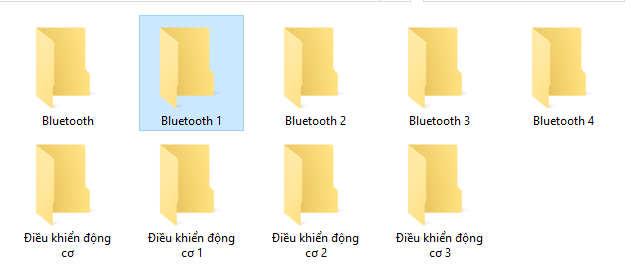
\includegraphics[width=1\linewidth]{images/DongCoBluetooth.PNG}
    \caption{Điều khiển động cơ}
\end{figure}

Sau đó anh kết hợp chúng lại với nhau để đủ chức năng hoàn chỉnh. May cho anh, sau một hồi code thì anh bắt đầu lên cơ và lần này thì không gặp phải vấn đề gì lớn lắm.

Chỉ nhớ gần đến này báo cáo thì anh bị mất máy tính, không cách nào lấy lại được dữ liệu của đồ án vừa mới làm, và phải chờ đến học kì sau.

\section{Quản lí sự thay đổi}

Do đặc tính của code là được chỉnh sửa, thêm mới, cải tiến, hiệu chỉnh... nói chung là thay đổi liên tục, Git được sinh ra để quản lí được sự thay đổi này.

Các bạn tải về theo đường link: https://git-scm.com/download/win.

Xem trước video mình demo cách hướng dẫn sử dụng git tại đường link:

Repository (gọi tắt là repo) là thư mục code được quản lí bởi git, ngoài những thư mục và file thông thường, một repo còn có một thư mục ẩn \textit{.git} để lưu thông tin.

Để sử dụng tốt Git thì ta cần hiểu rõ về chuyện gì đã xảy ra trong repo khi bạn gõ lệnh như \textit{git add, git commit, git push, git pull, git fetch}.

Đầu tiên ta có quy trình hoạt động của Git như sau:

\begin{figure}[h!]
    \centering
    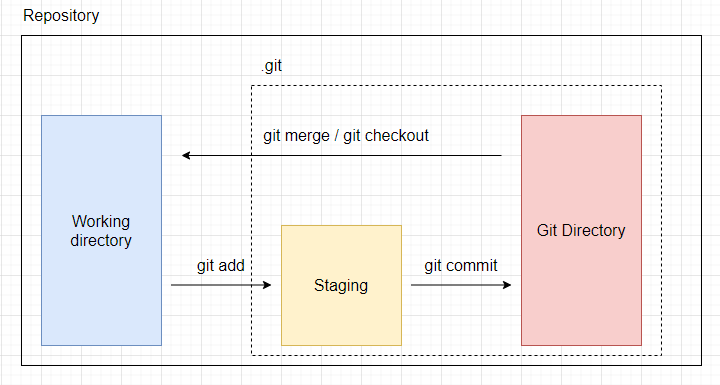
\includegraphics[width=1\linewidth]{images/gitCommitFlow.PNG}
    \caption{Git commit flow}
\end{figure}

Working directory là những file, folder mà ta có thể thấy và chỉnh sửa được. Những file trong Staging là những file chuẩn bị commit, và Git directory là nơi chứa dữ liệu sau khi commit.

Như tình huống anh sinh viên mỗi lần chỉnh sửa và test code của mình đều lưu ra một folder riêng \textit{bluetooth, bluetooth 1, blueotooth 2...}, thì tương tự mỗi commit sẽ lưu lại toàn bộ file và folder của bạn vào thư mục ẩn \textit{.git}, mỗi lần lưu như vậy gọi là một snapshot. Tuy nhiên Git có cơ chế riêng khiến việc lưu lại trở nên nhanh chóng và dễ dàng. Khi cần ta có thể lấy code ở một commit bất kì ra Working directory và phát triển tiếp.

Ngoài việc lưu lại code, git còn giúp ta có thể xem lại những thông tin chi tiết của mỗi lần commit, xem lần đó đã thay đổi những file nào, và từng file thì thay đổi phần nào.

\Section{Quản lí tập trung}

Như trường hợp anh sinh viên bị mất máy tính ở trên, việc lưu công sức lao động của mình trên máy tính thật sự rất nguy hiểm, nhất là những dự án cần có công sức của nhiều người và làm việc trong nhiều năm.

Các trang như Github, Gitlab, Gitbucket ra đời cho phép bạn lưu code của bạn lên các trang này, với độ đảm bảo tin cậy hơn rất nhiều so với máy tính cá nhân. Các trang này đều sử dụng Git làm nền tảng, việc upload hoặc download code rất đơn giản chứ không rườm rà như việc bạn nén folder code lại và lưu trên google drive hoặc one drive. Ngoài ra git còn hỗ trợ tốt cho việc làm việc với nhiều người, giữa nhiều tổ chức với nhau, nhưng ở đây mình chỉ đề cập đến khía cạnh làm việc cá nhân.

Các bạn xem video mình demo cách sử dụng Git để lưu trữ code lên Github.

